\chapter{Background}
\label{chp:background} 

\section{Village Telco}
%How did it all start?

\section{Mesh Potato}
%Generelt om MP

% hvordan MPen fikk navnet. 

\begin{figure}[h!]
  \centering
      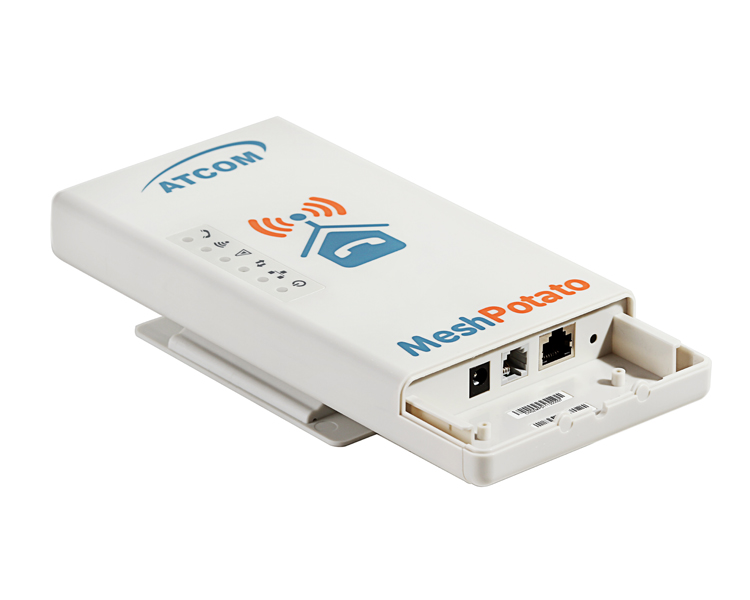
\includegraphics[width=0.5\textwidth]{MP01}
  \caption [The Mesh Potato]{\textbf{The fist generation Mesh Potato, MP01}}
  \label{fig:MP01}
\end{figure}

%MP01
The Mesh Potato, as shown in \fref{MP01}, is designed to be used in rural areas. It can be deplyed and run anywhere in the world relying only on a low, but stable power supply. The ethernet port, Foreign eXchange Station (FXS) ports and power are robust and designed to handle hard weather, poor power conditions, lightening and static electricity. In addition the Mesh Potato comes in a waterproof box for outdoor mounting \cite{background}.

The Mesh Potato combines the features of a 802.11bg WiFi router with an Analog telephone Adaptor (ATA) \cite{MP}. Each Mesh Potato provies a single fixed telephone line to the end user. The MPs are connected together via a mesh WiFi network, and  configure themselves automatically to form a peer-to-peer network, greatly extending the range of the network over regual WiFi. Enabling phone calls to be made independent of landlines and telephone towers. Creating the basis for the "plug-and-play" solution. 








The Mesh network can be connected vi a backbone link to the rest of the world by using VoIP trunks. 


MP02





\section{Technology}

\subsection{Ad Hoc and Mesh Networks}
%Eksempel på nettverk
\subsection{OpenWrt}


\section{The Cost Structure and Revenue Model(s) of Village Telco Today}

\section{Comparison of Village Telco and Other Telcos}

\section{Refugee Camps}
\subsection{The Existing Communication Methods}